\section{Methodology}
\label{sec:method}
MidCache implements the encoder--cache--reader view within one decoder: the lower prefix encodes document chunks for persistent reuse, and the upper suffix reads selected encodings with the current query. Both parts use the original transformer blocks.
\begin{figure}[t]
\centering
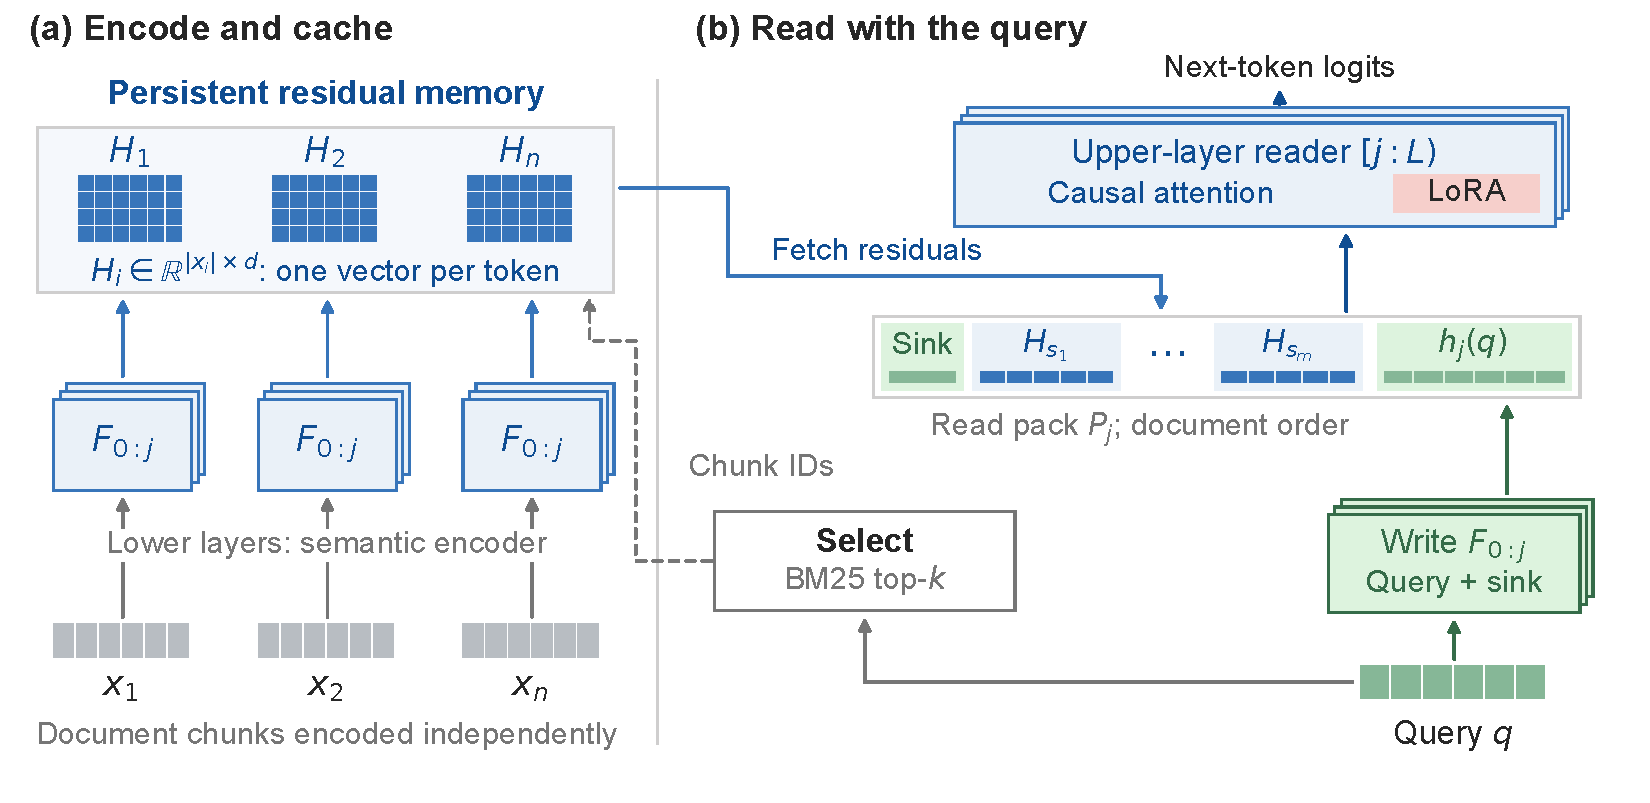
\includegraphics[width=\linewidth]{figures/architecture.pdf}
\caption{\textbf{CoMem reuses document computation at a residual interface.} (a) The shared lower-layer semantic encoder writes each chunk into a residual matrix $H_i$. (b) The query selects at most $k$ chunk IDs (dashed path). Cached encodings (blue) join separately encoded sink/query states (green), in document order, for causal processing by the upper reader $[j{:}L)$. Suffix LoRA adapts this reader to independently written states; the frozen variant omits it. Overlap-Write adds left context in (a) while retaining only target-token states.}
\label{fig:arch}
\end{figure}

Let a decoder have $L$ blocks, hidden width $d$, and half-open layer ranges. The residual $h_j$ is the input to block $j$, after blocks $[0{:}j)$ have run. A document of $N$ tokens is divided into chunks $x_i$ of at most $c$ tokens. The split $j$, chunk size $c$, and retrieval budget $k$ define the reusable interface.

\paragraph{Choosing the split.}
The principal Qwen3-8B configuration uses $j=12$, prepaying 12 of 36 blocks and leaving 24 for Read. Section~\ref{sec:depth-choice} explains this operating choice with a depth sweep; Appendix~\ref{app:split-choice} specifies the implementation's default rule.

\subsection{Write once, Read across queries}
\label{sec:interface}
\paragraph{Write: cache the semantic encoder's output.}
For $j>0$, each chunk is processed independently with rotary positions restarted at zero. We retain $H_i=F_{0:j}(x_i)\in\mathbb{R}^{|x_i|\times d}$, where $F_{0:j}$ denotes the embedding and lower-block computation. This is one vector \emph{per token}. A separate token-ID BM25 index maps the question to chunk IDs, which address the stored residuals. At $j=0$, the stored object is token IDs and document computation is deferred to each query.

\paragraph{Retrieval policy.}
The principal selector uses deterministic token-ID BM25 \citep{bm25}, top-12 chunks, hop width four, and three frontier-expansion rounds. The first round scores the question; subsequent rounds use newly selected chunks as the query frontier, deduplicate IDs, and break ties by document index. Retrieval uses CPU lookups without model forward passes; it addresses the cached states through chunk IDs rather than comparing residual vectors directly.

\paragraph{Select and Read: continue through the upper reader.}
Given a question, the selector returns at most $k$ chunk IDs, sorted back into document order. Let $q$ be the online query segment and $s$ the one-token sink. For $j>0$, both are encoded through the lower blocks independently of the stored chunks. The reader constructs
\begin{equation}
 P_j=[h_j(s);\,H_{s_1};\ldots;H_{s_m};\,h_j(q)],
 \qquad m\leq k,
 \label{eq:pack}
\end{equation}
and executes $F_{j:L}$ with fresh contiguous Read positions. Attention is causal: later chunks use earlier chunks, and query tokens use all selected chunks. Earlier document tokens do not attend to the later query. Each generated token still traverses all $L$ layers: lower-layer KV covers $q$ and the generated prefix, while upper-layer KV covers the selected pack and generated prefix. These KV caches are request-local; only document residuals persist across queries. Appendix~\ref{app:query-boundary} specifies benchmark query boundaries and sink conventions.

The matched $j=0$ reader assembles the same sink, chunk tokens, and query with the same order and causal mask, then executes the entire decoder. For the principal depth comparison, both endpoints carry the same suffix LoRA. Consequently, the comparison isolates the deployed depth interface without changing the selected evidence or adaptation parameters. It does not assume that independently written $h_j$ equals a continuous-prefix residual.

\paragraph{Relation to prefill and decode.}
Write--Read describes cross-query reuse. Online Read prefills the assembled states through the upper layers before autoregressive decode; it saves repeated document encoding, while generated tokens still use the complete decoder. Section~\ref{sec:infra} and Appendix~\ref{app:systems} distinguish this saved prefill work from TTFT and Write-inclusive E2E.

\paragraph{Storage and model-side work.}
For element size $b$, head width $d_{\mathrm{head}}$, $n_{\mathrm{kv}}$ KV heads, and $n_{\mathrm q}$ query heads, residual and full-KV bytes per token are $bd$ and $2bLn_{\mathrm{kv}}d_{\mathrm{head}}$. With $d=n_{\mathrm q}d_{\mathrm{head}}$,
\begin{equation}
 \frac{\mathrm{residual\ bytes/token}}{\mathrm{full\ KV\ bytes/token}}
 =\frac{d}{2Ln_{\mathrm{kv}}d_{\mathrm{head}}}
 =\frac{n_{\mathrm q}}{2Ln_{\mathrm{kv}}}.
 \label{eq:storage}
\end{equation}
For Qwen3-8B in bf16, this is 8 KiB versus 144 KiB per token. Residual bytes are independent of $j$ for the nonzero splits studied here; deeper caching changes prepaid computation, not tensor width. The $j=0$ token-ID endpoint is much smaller. The online pack length is bounded by $1+kc+|q|$, so model-side Read work is independent of $N$ for fixed $k,c,|q|$. Decode additionally depends on the generated prefix. Write, persistent storage, indexing, and selection still grow with the corpus.

\subsection{Adapt the suffix to independently written states}
\label{sec:distill}
The cached states encode document content, but independent Write changes the context seen below the split. We therefore train the reader to consume this interface using rank-32 LoRA on attention and MLP projections in blocks 12--35 of frozen Qwen3-8B \citep{lora,qwen3}. A $j=12$ student matches an adapter-disabled $j=0$ teacher on plain PG-19 windows \citep{pg19,distillation}. Each window supplies seven context chunks and a query chunk. The teacher processes the complete ordered pack causally through all layers. The student encodes each chunk, the sink, and the query independently below the split, then processes their assembled states causally in the adapted suffix. Both use the same token IDs and order; neither sees future tokens. Only query tokens contribute to the loss.

At token $t$, let $S_t$ contain the teacher's top-64 vocabulary indices. Teacher probabilities $p_t$ and student probabilities $q_t$ are separately renormalized on this same support. The token-mean objective is
\begin{equation}
 \mathcal{L}=\frac{1}{|Q|}\sum_{t\in Q}
 \left[0.6\,\mathrm{KL}(p_t\Vert q_t)+0.4\,\mathrm{KL}(q_t\Vert p_t)\right],
 \label{eq:distill}
\end{equation}
where $Q$ denotes query-token positions. This matches the conditional distributions on $S_t$, without constraining the student's total probability mass on that support. Post-training validation measures retained mass and full-vocabulary divergence (Appendix~\ref{app:distillation-validation}). Training uses 4,000 steps on 4,096-token windows, without retrieval, synthetic long-context data, or benchmark supervision. Appendix~\ref{app:protocol} specifies visibility, positions, and optimization. The adapter-disabled training teacher is distinct from the adapter-matched evaluation endpoint.

All full-suite results use independently written, nonoverlapping chunks. To diagnose sensitivity to encoding context, a separate Overlap-Write variant adds a short left prefix during Write and discards its states (Appendix~\ref{sec:overlap}); Section~\ref{sec:diagnosis} reports its quality and cost.
